\begin{frame}
  \begin{tikzpicture}[remember picture,overlay]
    \fill [white] (current page.south west) rectangle (current page.north east);
    \node at (current page.center) {\resizebox{!}{\textheight}{ \begin{tikzpicture}
\newcommand\XLabel{7}
\newcommand\XNode{10}
\newcommand\XEngines{14}
\newcommand\TextWidth{3}
\tikzset{>=latex}

%\draw[help lines] (5,5) grid (15,20);

%%%%%%%%%%%% MID STRUCTURE %%%%%%%%%%%%%%%%%%%
\node[inner sep=10pt] (code) at (\XNode,18)
    {
\includegraphics[width=.1\textwidth]{./graphics/implementation_overview_images/source_code.png}};
\node[text width=\TextWidth{}cm] at (\XLabel,18) {\hfill{}Source code};

\node[inner sep=10pt] (ast) at (\XNode,15)
    {
\includegraphics[width=.15\textwidth]{./graphics/implementation_overview_images/ast.png}};
\node[text width=\TextWidth{}cm] at (\XLabel,15) {\hfill{}AST};

\node[inner sep=10pt] (cfg) at (\XNode,11)
    {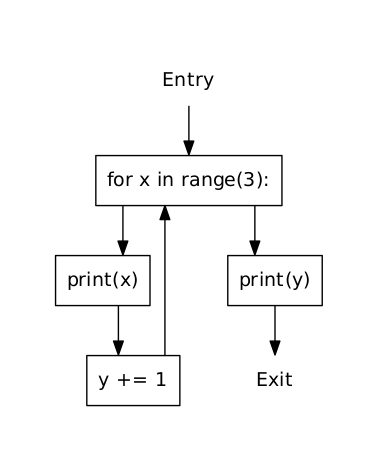
\includegraphics[width=.2\textwidth]{./graphics/implementation_overview_images/for_complete.png}};
\node[text width=\TextWidth{}cm] at (\XLabel,11) {\hfill{}CFG};

\node[inner sep=10pt] (engine) at (\XNode,7)
    {
\includegraphics[width=.1\textwidth]{./graphics/implementation_overview_images/cog_wheel.png}};
\node[text width=\TextWidth{}cm] at (\XLabel,7) {\hfill{}Framework \\ \hfill{}Adaptor};

\node[inner sep=10pt] (algorithm) at (\XNode,4)
    {
\includegraphics[width=.1\textwidth]{./graphics/implementation_overview_images/spiral.png}};
\node[text width=\TextWidth{}cm] at (\XLabel,4) {\hfill{}Fixed Point \\ \hfill{}Algorithm};

\node[inner sep=10pt] (vulnerabilities) at (\XNode,1)
    {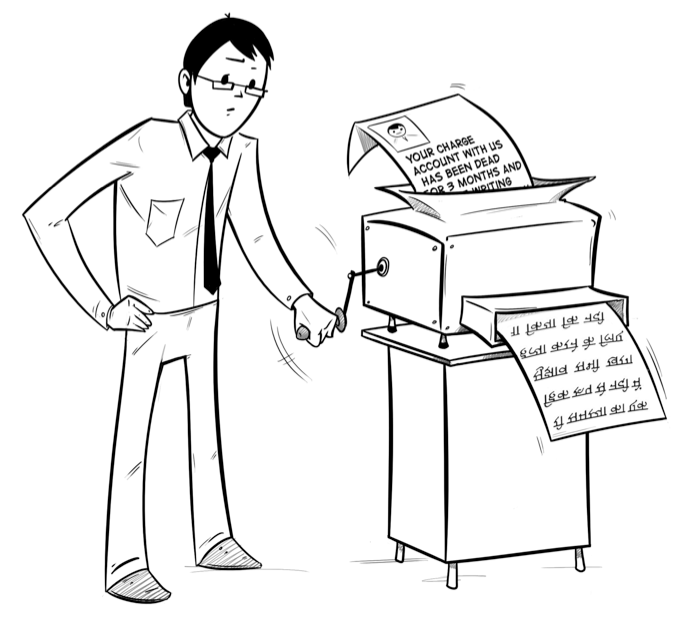
\includegraphics[width=.15\textwidth]{./graphics/implementation_overview_images/vulnerability.png}};
\node[text width=\TextWidth{}cm] at (\XLabel,1) {\hfill{}Vulnerabilities};
\draw[red, very thick] (\XNode-1.25, 1) ellipse (3cm and 1.25cm);

%%%%%%%%%%%%%%%%%%%% Adaptors %%%%%%%%%%%%%%%%%%%%%%%%
\node[inner sep=10pt] (flask) at (\XEngines,11)
    {
\includegraphics[width=.2\textwidth]{./graphics/implementation_overview_images/flask_text.png}};

\node[inner sep=5pt] (django) at (\XEngines,9)
    {
\includegraphics[width=.13\textwidth]{./graphics/implementation_overview_images/django.png}};

\node[label=below:{Other}, inner sep=5pt] (other_engine) at (\XEngines,7)
    {
\includegraphics[width=.05\textwidth]{./graphics/implementation_overview_images/question_mark.png}};

%%%%%%%%%%%%%%%% ANALYSIS %%%%%%%%%%%%%%%%%%%%%%%%%    
\node[label=below:{Analysis}, inner sep=10pt] (analysis) at (\XEngines,4)
    {
\includegraphics[width=.1\textwidth]{./graphics/implementation_overview_images/analysis.png}};

\node[text width=2cm, inner sep=10pt] (reaching) at (18,7) {Reaching Definitions};
\node[text width=2cm, inner sep=10pt] (liveness) at (18,4) {Liveness};

\node[label=below:{Other}, inner sep=5pt] (other_analysis) at (18,1)
    {
\includegraphics[width=.05\textwidth]{./graphics/implementation_overview_images/question_mark.png}};


\draw[->] (code) -- (ast);
\draw[->] (ast) -- (cfg);
\draw[->] (cfg) -- (engine);
\draw[->] (engine) -- (algorithm);
\draw[->] (algorithm) -- (vulnerabilities);

\draw[->] (flask) -- (engine);
\draw[->] (django) -- (engine);
\draw[->] (other_engine) -- (engine);

\draw[<->] (algorithm) -- (analysis);
\draw[->] (reaching) -- (analysis);
\draw[->] (liveness) -- (analysis);
\draw[->] (other_analysis) -- (analysis);

\end{tikzpicture}}};
  \end{tikzpicture}
\end{frame}

\begin{frame}[fragile]{Sources and Sinks}
  Sources and sinks are identified by 'trigger words'
  \begin{lstlisting}[style=default, escapeinside={(*@}{@*)}]
sources:
get(
form[
Markup(
(*@{\color{red}.data}@*)

sinks:
replace( -> escape
send_file( -> '..', '..' in
execute(
filter(
subprocess.call(
\end{lstlisting}

\end{frame}

\begin{frame}{Identifying triggers in CFG}
  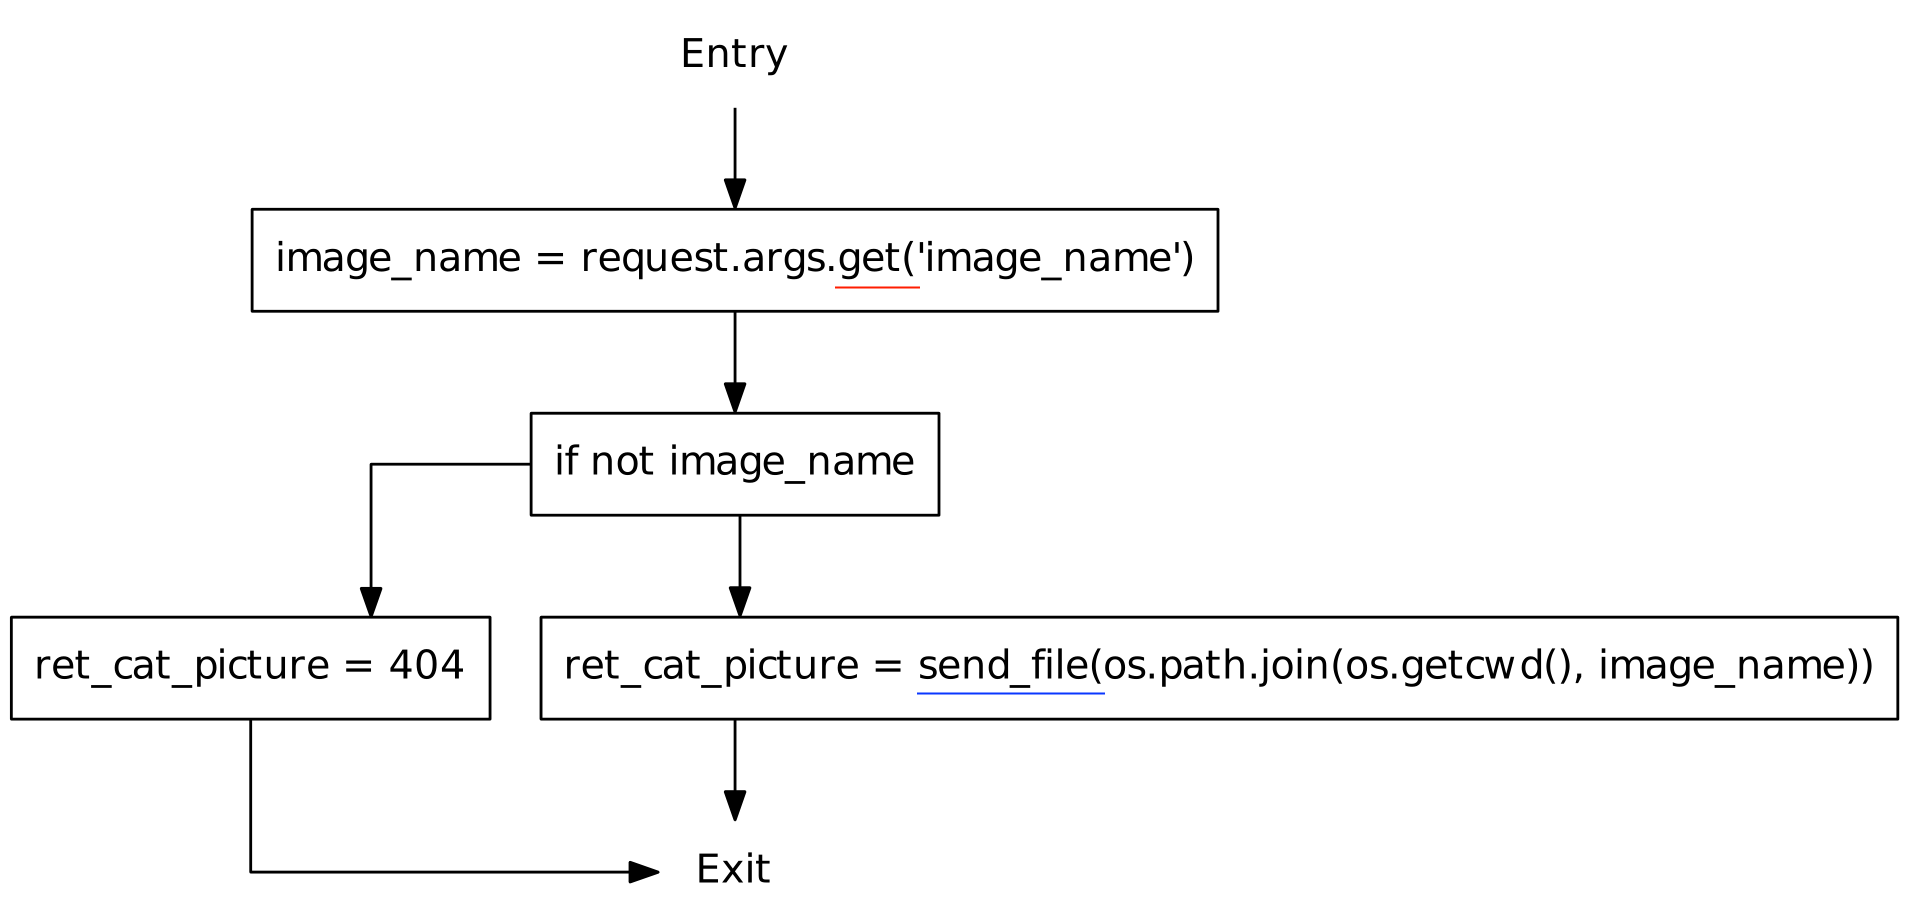
\includegraphics[width=1.05\textwidth]{graphics/cfg_path_traversal_triggers}
\end{frame}

\begin{frame}{Looking up the nodes}
\[
\begin{array}{lclcl}
  \constraint{entry} & = & \{\} &&\\
  \assignconstraint{image} & = & \{image\} &&\\
  \constraint{if} & = & \{image\} &&\\
  \constraint{ret\_404} & = & \{ret\_404, image\} &&\\
  \assignconstraint{ret\_send} & = & \{ret\_send, image\} &&\\
  \constraint{exit} & = & \{ret\_send, ret\_404, image\} &&\\
  && \phantom{\{command, param\}} && \phantom{\{command, param\}}
\end{array}
\]
\end{frame}
